%\VignetteIndexEntry{Introduction to SpaDES: A package to develop and run spatially explicit discrete event simulation models.}
%\VignetteDepends{SpaDES}
%\VignetteKeyword{discrete event simulation}
\documentclass{article}

%%% latex packages
\usepackage[T1]{fontenc}
\usepackage{hyperref}
\usepackage[utf8]{inputenc}
\usepackage[usenames,dvipsnames]{xcolor}

%% change margins to 1" all the way around
\oddsidemargin 0.0in
\evensidemargin 0.0in
\textwidth 6.5in
\headheight 0.0in
\topmargin 0.0in
\textheight 9.0in

%%% document info
\title{Introduction to \texttt{SpaDES}}

\author{
  Alex M. Chubaty\\
	\small{Natural Resources Canada, Pacific Forestry Centre}\\
	\small{email: \href{mailto:achubaty@nrcan.gc.ca}{achubaty@nrcan.gc.ca}}
	\and
	Eliot McIntire\\
	\small{Natural Resources Canada, Pacific Forestry Centre}\\
	\small{email: \href{mailto:emcintir@nrcan.gc.ca}{emcintir@nrcan.gc.ca}}
}

\usepackage{Sweave}
\begin{document}
\Sconcordance{concordance:introduction.tex:introduction.Rnw:%
1 31 1 1 0 14 1 1 3 2 0 1 1 1 10 8 0 1 2 7 0 1 5 14 1 1 2 1 0 4 1 1 2 4 %
0 1 2 22 1 1 2 1 0 1 4 2 0 1 2 1 0 3 1 1 5 3 0 1 1 1 2 11 0 1 1 15 0 1 %
7 5 0 1 2 5 0 1 2 7 1}

 % displays code as entered (no arranging lines)

\maketitle

\abstract{Easily implement a variety of simulation models, with a focus on spatially explicit agent based models. The core simulation components are built upon a discrete event simulation framework that facilitates modularity, and easily enables the user to include additional functionality by running user-built simulation modules. Included are numerous tools to visualize raster and other maps.\\
\\
\textbf{Website:} \url{https://github.com/achubaty/SpaDES}}

\tableofcontents

\newpage

\section{Introduction}

\subsection{Objectives and motivations}

\paragraph{}
We have been building spatial simulation models for several years and got tired of rebuilding the wheel every time. So, we had been looking for a generic platform that could be used to make new models quickly, and provide a link to existing models, so that an already well described and mature model, can be used with a \textit{de novo} one. Or better yet, use several \textit{de novo} models and several existing models in combination. This approach requires a platform that allows for modular reuse of models (herein called ``modules'') as hypotheses that can be evaluated and tested in various ways.

\begin{enumerate}
  \item Allow rapid building of models of a wide diversity of types (IBMs, raster models, differential equation models etc.).
  \item Run faster and more memory efficiently than current systems for doing similar things (NetLogo, SELES, Repast etc.).
  \item Take advantage of R's strengths as a data platform, its capabilities to call external software such as databases, its excellent visualization and graphics, and its abilities for high performance computing. We don't have to implement all of these from scratch ourselves!
  \item Be open source, but also make it as easy as possible for many people to easily contribute modules and code. In particular, to make it easy for scientists already familiar with R but who aren't formally trained as computer programmers.
  \item \texttt{SpaDES} is built around modularity so that models can be seen as modules that are easily replaceable, not just ``in theory'' replaceable.
  \item Allow tight coupling between data and model simulations so that calibration is not actually something that one has to redesign every time there is a new data set.
\end{enumerate}

\subsection{Discrete event simulation and \texttt{SpaDES}}

\paragraph{}
Discrete event simulation is...

event driven: an activity changes the state of the system at particluar times. a particular activity may have several events assoriated with it. future events are scheduled in an event queue, and then processed in order.

rather than advancing time in fixed increments, time advances to the time of the next event in the queue (assume that state of the system only changes due to events, therefore no change between events, so no need to run the clock).

\paragraph{}
`time` as the core concept linking simulation components: activities schedule events (i.e. change the system according to their programmed rules) and do not need to know about each other, which allows for modularity of simulation components. thus, complex simulations involving multiple processes (activities) can be build fairly easily, provided these processes are modelled using a common DES framework.

\paragraph{}
\texttt{SpaDES} provides such a framework, facilitating interaction between multiple processes (built as ``modules'') that don't interact with one another directly, but are scheduled in the event queue and carry out operations on shared data objects in the global simulation evnivironment. This package provides tools for easily building modules natively in \textsf{R} that can be reused; however, because of the flexibilty R provides for interacting with other programming langugages and external datasources, modules can also be built using external tools.

\begin{figure}[!htbp]
  \centering
	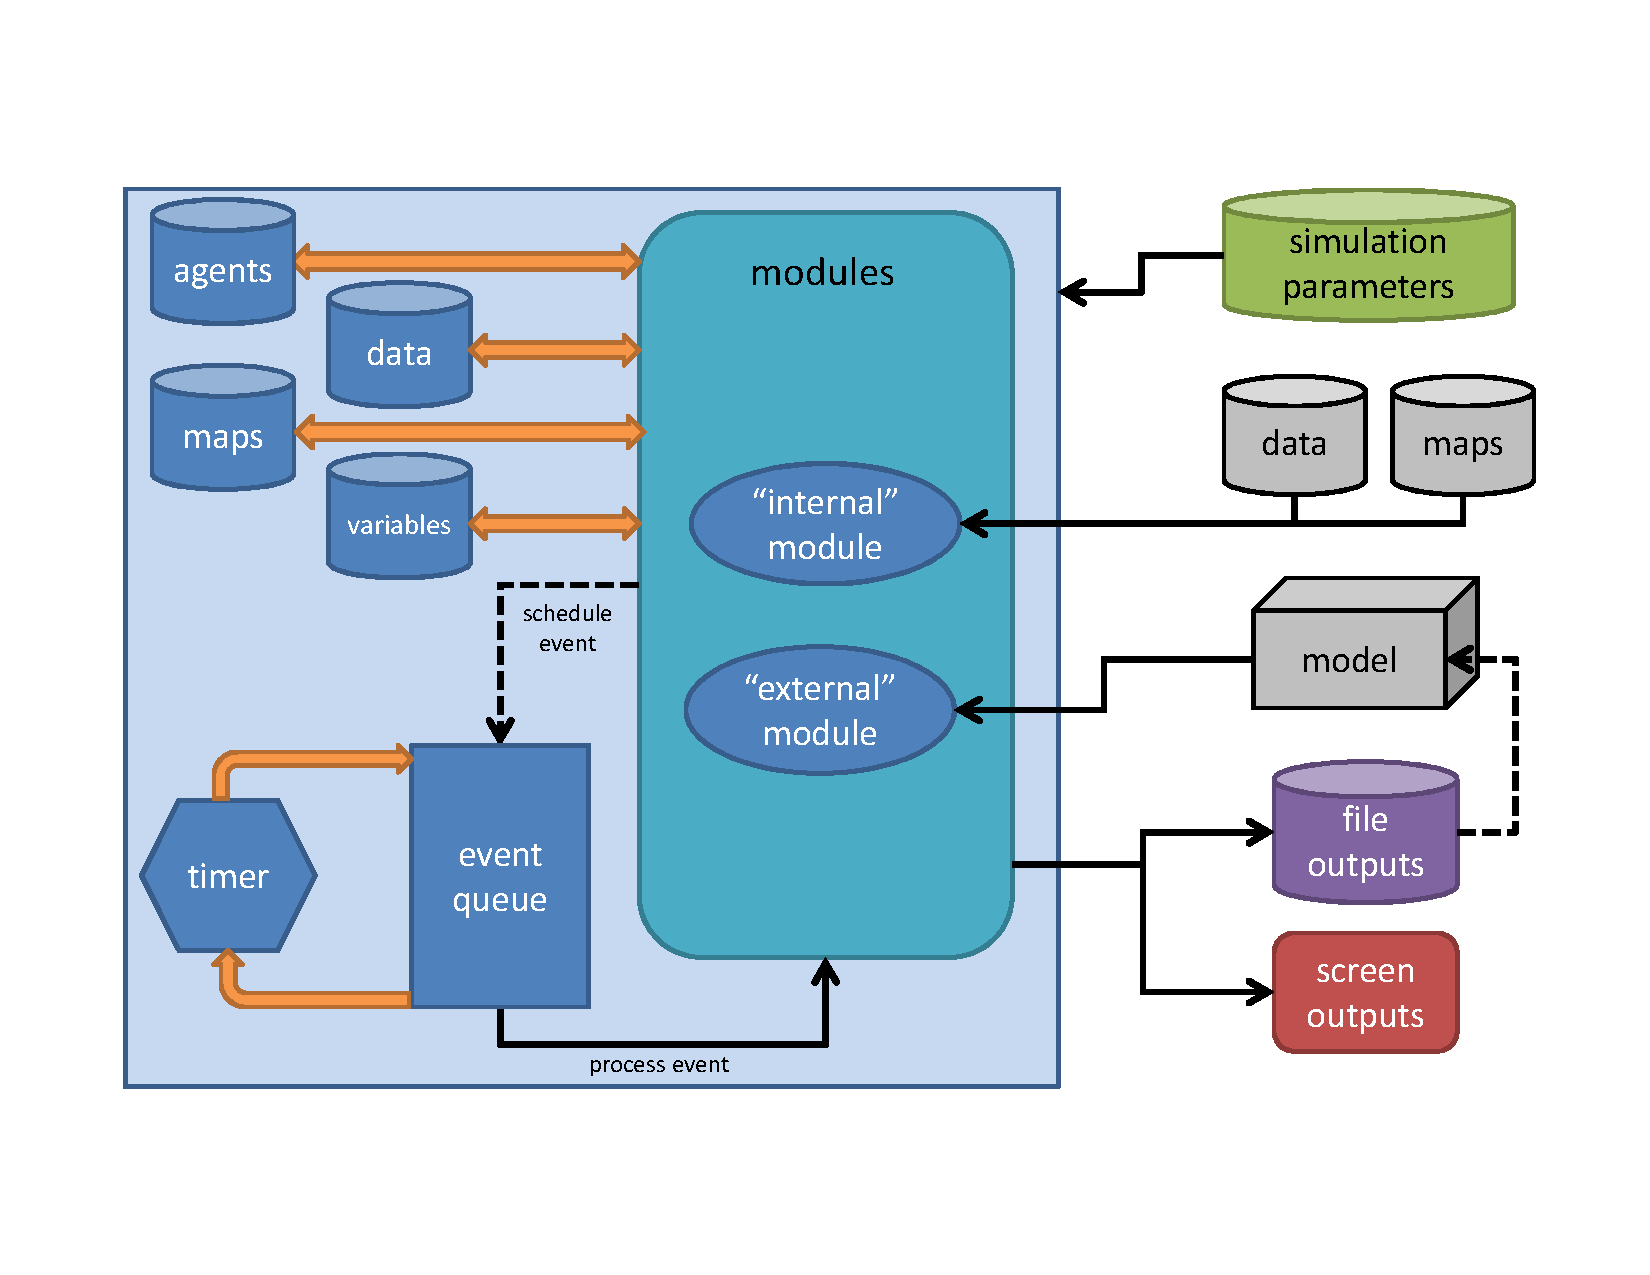
\includegraphics[width=5in]{../inst/SpaDES-overview-diagram.pdf}
	\caption{Schematic representation of a \texttt{SpaDES} simulation model.}
	\label{figure-SpaDES-overview}
\end{figure}

\subsection{\texttt{SpaDES} demos and sample modules}

\paragraph{}
The static nature of PDFs does not allow us to really show off the simulation visualization components of this package, so we invite you to check out the included demos, to run the sample simulation provided in this vignette, and to view the source code for the sample modules included in this package.

\subparagraph{Demos:}

\begin{Schunk}
\begin{Sinput}
> library("SpaDES")
> # demo: randomLandscapes, fireSpread, caribouMovement
> demo("spades-simulation", package="SpaDES")
\end{Sinput}
\end{Schunk}

\subparagraph{Sample model:}

\begin{Schunk}
\begin{Sinput}
> library("SpaDES")
> .cols[[5]] <- c("#FFFFFFFF", rev(heat.colors(9)))
> outputPath=file.path("~", "tmp", "simOutputs")
> times <- list(start=0,stop=100)
> parameters <- list(.globals=list(mapName="landscape", .outputPath=outputPath,
+                                  burnStats="nPixelsBurned"),
+                    .progress=list(NA),
+                    randomLandscapes=list(nx=1e2, ny=1e2, inRAM=TRUE),
+                    fireSpread=list(nFires= 1e1, spreadprob=0.225, its=1e6,
+                                    persistprob=0, returnInterval=10, startTime=0,
+                                   .plotInitialTime=0.1, .plotInterval=10),
+                    caribouMovement=list(N=1e2, moveInterval=1,
+                                         .plotInitialTime=1.01, .plotInterval=1)
+                    )
> modules <- list("randomLandscapes", "fireSpread", "caribouMovement")
> path <- system.file("sampleModules", package="SpaDES")
> mySim <- simInit(times=times, params=parameters, modules=modules, path=path)
> spades(mySim)